% !TeX program = lualatex
% ================================================================
% Polish Parallel Text Version of SequencesAndEquationsExtension
%
% Generated by the server using the following settings:
%
%   language            Polish (pol)
%   text direction      left to right
%   font                Noto Serif
%   fallback font       Noto Serif
%   built from          latex/worksheets/sequences/sequencesAndEquationsExtension.tex
%   vocabulary key      latex/worksheets/sequences/sequencesAndEquationsExtension/L2/pol/sequencesAndEquationsExtension_polishKey.tex
%   tier 3 vocabulary   green   RGB 0 128 0
%   English text        black   RGB 0 0 0
%   Polish text         purple  RGB 112 48 160
%   layout macros       version 3
%
% Please don't edit any information in this comment block - the server
% compares it against the current settings and rebuilds this file when
% they differ, so changes here would be overwritten. However, feel free
% to make updates to the LaTeX below if you want to edit it.
% ================================================================

\documentclass[11pt,a4paper]{article}
% ================================================================
% Copied from the English sheet this was translated from, so that
% anything it sets up for itself still works here
% ================================================================
\usepackage[a4paper,top=10mm,bottom=10mm,left=14mm,right=14mm]{geometry}
\usepackage[T1]{fontenc}
\usepackage{amsmath}
\usepackage{amssymb}
\usepackage{enumitem}
\usepackage{multicol}
\usepackage{array}
\usepackage{tikz}
\usepackage[most]{tcolorbox}
\usetikzlibrary{arrows.meta,decorations.pathreplacing}

% ================================================================
% Sequences and equations: an extension sheet.
%
% For pupils who can find the nth term of a linear sequence and solve
% linear equations. Every equation on the sheet comes from a question
% about sequences, and each part brings in one kind of equation.
%
% Part 1 sets two nth terms equal to find where two sequences meet,
% which puts the unknown on both sides: two candles burning down, and
% one phone running down while another charges. It ends with sequences
% that never meet.
%
% Part 2 compares terms in different positions, which gives brackets:
% three terms of a linear sequence written in x, rows of matchstick
% houses beside rows of squares and triangles with more shapes in
% them, a fence with one more post than panels, and cells that triple
% each hour.
%
% Part 3 has sequences with n in the denominator: a minibus cost shared
% between n people, a pizza cut into n slices, the fraction of a garden
% path that is grey, a sequence of fraction bars, and a minibus and a
% coach that cost the same for each person.
%
% Part 4 finds an unknown nth term an+b from two of its terms, which
% gives simultaneous equations: stacks of cups and of chairs, two
% sequences an+5 and bn+6, the fence again, and a Fibonacci-type
% sequence. It ends with open tasks.
%
% Each part starts with a worked example, followed by the same layout
% with gaps, and then by questions with the layout taken away.
% Equations are solved by doing the same thing to both sides, with the
% operation written under both sides, never with a flow chart.
% Simultaneous equations are solved by elimination.
%
% n is a position in a sequence, so a solution that is not a positive
% whole number shows that a number is not a term, or that two
% sequences never have equal terms in the same position. Several
% questions turn on this.
%
% The answers are in a comment beside each question. Every picture is
% drawn from its numbers, so the pictures agree with the answers.
% The sheet is written on and is six sides of A4.
% ================================================================

\pagestyle{empty}
\setlength{\parindent}{0pt}
\setlength{\parskip}{3pt}
\setlength{\multicolsep}{3pt}
\setlength{\columnsep}{14pt}
\setlist[enumerate,1]{label=\textbf{Q\arabic*.}, leftmargin=*, itemsep=6pt, topsep=4pt, parsep=2pt}
\setlist[enumerate,2]{label=(\alph*), leftmargin=*, itemsep=4pt, topsep=3pt, parsep=1pt}
\newcolumntype{C}[1]{>{\centering\arraybackslash}m{#1}}

% A gap for one number in a sentence, and a longer line for an answer.
\newcommand{\gap}{\underline{\hspace{0.95cm}}}
\newcommand{\ansline}[1][2.2cm]{\underline{\hspace{#1}}}
% Space to work in, ending with a line for the answer.
\newcommand{\workspace}[1]{\par\vspace{#1}\hfill Answer: \ansline[3.5cm]\par}
% The strut that sets the height of a table row to be written in.
\newcommand{\rowstrut}{\rule[-1.9mm]{0pt}{5.8mm}}

% The idea each part is built on, stated once and boxed, and the
% worked example. The boxes are tinted only faintly, and the title bar
% is pale with coloured text, so that the sheet is cheap to print.
\newtcolorbox{keyidea}{colback=orange!3,colframe=orange!35,boxrule=0.6pt,
  left=6pt,right=6pt,top=3pt,bottom=3pt}
\newtcolorbox{wex}[1]{colback=blue!2,colframe=blue!30,boxrule=0.6pt,
  colbacktitle=blue!8,coltitle=blue!50!black,
  left=6pt,right=6pt,top=3pt,bottom=4pt,
  title={\bfseries\small Worked example: #1},fonttitle=\small,
  toptitle=1pt,bottomtitle=1pt}

% The section headings, kept tight so the parts do not eat the page.
\newcommand{\parttitle}[2]{%
  \vspace{1pt}
  {\color{blue!45!black}\rule{\linewidth}{1pt}}\\[1pt]
  {\large\bfseries Part #1: #2}\\[-6pt]
  {\color{blue!45!black}\rule{\linewidth}{0.4pt}}
  \par\vspace{-5pt}}

% ----------------------------------------------------------------
% Working for an equation solved by doing the same thing to both
% sides. The lines are lined up on the equals sign. Between two lines,
% \bsop writes the operation under both sides, \bsopgap leaves both
% operations blank to fill in, and \bsnote writes a step that changes
% the whole line, such as expanding brackets. \sidegap is a blank for
% one side of a line.
\newenvironment{working}
  {\(\renewcommand{\arraystretch}{1.06}\begin{array}{@{}r@{\;}c@{\;}l@{}}}
  {\end{array}\)}
\newcommand{\opstyle}[1]{\text{\footnotesize\color{blue!55!black}$#1$}}
\newcommand{\bsop}[1]{\opstyle{#1} & & \opstyle{#1}\\}
\newcommand{\opgap}{\rule{0pt}{4.3mm}\rule{0.9cm}{0.4pt}}
\newcommand{\bsopgap}{\opgap & & \opgap\\}
\newcommand{\bsnote}[1]{\multicolumn{3}{c}{\text{\footnotesize\color{blue!55!black}#1}}\\}
\newcommand{\sidegap}[1][1.7cm]{\rule{0pt}{5.3mm}\rule{#1}{0.4pt}}

% A worked example or question laid out with a picture or table on the
% left, the working on the right and a sentence underneath:
% \eqlayout{<left width>}{<left>}{<working>}{<sentence>}
\newcommand{\eqlayout}[4]{%
  \begin{minipage}[c]{#1\linewidth}\raggedright #2\end{minipage}\hfill
  \begin{minipage}[c]{\dimexpr0.98\linewidth-#1\linewidth\relax}\centering #3\end{minipage}\par\smallskip
  #4}

% The layout of Part 1, with the table of terms and the sentence under
% it on the left, and the working on the right:
% \meetlayout{<table>}{<working>}{<sentence>}
\newcommand{\meetlayout}[3]{%
  \begin{minipage}[c]{0.62\linewidth}\raggedright #1\par\medskip #3\end{minipage}\hfill
  \begin{minipage}[c]{0.36\linewidth}\centering #2\end{minipage}}

% ----------------------------------------------------------------
% Part 1. The terms of two sequences in positions 1 to 8, one sequence
% to a row. \termtable[<header>]{<name>}{<8 terms>}{<name>}{<8 terms>},
% with the terms separated by &. \hl shades a cell, to show where the
% two sequences meet.
\newcommand{\hl}[1]{\cellcolor{orange!18}#1}
\newcommand{\termtable}[5][1 & 2 & 3 & 4 & 5 & 6 & 7 & 8]{%
  {\setlength{\tabcolsep}{2pt}%
  \begin{tabular}{|C{1.95cm}|*{8}{C{0.72cm}|}}\hline
  {\small Position $n$} & #1\\\hline
  #2\rowstrut & #3\\\hline
  #4\rowstrut & #5\\\hline
  \end{tabular}}}

% A candle h cm tall, with its base at (x,0), drawn 1 cm to 0.07 cm:
% \candle{<x>}{<h>}{<name>}
\newcommand{\candle}[3]{%
  \begin{scope}[shift={(#1,0)}]
  \pgfmathsetmacro{\ch}{0.062*#2}
  \draw[fill=yellow!8,line width=0.5pt] (-0.16,0) rectangle (0.16,\ch);
  \draw (0,\ch) -- (0,\ch+0.08);
  \fill[orange!55] (0,\ch+0.05) .. controls (0.1,\ch+0.14) and (0.06,\ch+0.26) .. (0,\ch+0.34)
    .. controls (-0.06,\ch+0.26) and (-0.1,\ch+0.14) .. (0,\ch+0.05);
  \node[font=\scriptsize,above,inner sep=1pt] at (0,\ch+0.34) {#2\,cm};
  \node[font=\scriptsize,below,inner sep=2pt] at (0,0) {#3};
  \end{scope}}
% Candles A and B after a number of hours, on a shelf:
% \candlepair{<x>}{<hours>}{<height of A>}{<height of B>}
\newcommand{\candlepair}[4]{%
  \begin{scope}[shift={(#1,0)}]
  \draw[line width=0.8pt] (-0.42,0) -- (1.32,0);
  \candle{0}{#3}{A}\candle{0.9}{#4}{B}
  \node[font=\scriptsize\bfseries] at (0.45,-0.62) {After #2};
  \end{scope}}

% A phone battery that is p% charged, with its bottom left corner at
% (x,y): \battery{<x>}{<y>}{<p>}
\newcommand{\battery}[3]{%
  \begin{scope}[shift={(#1,#2)}]
  \draw[line width=0.6pt,rounded corners=1.5pt] (0,0) rectangle (1.1,0.42);
  \fill (1.1,0.12) rectangle (1.17,0.30);
  \fill[gray!30] (0.05,0.05) rectangle ({0.05+0.01*#3},0.37);
  \node[font=\scriptsize] at (0.55,0.21) {#3\%};
  \end{scope}}

% ----------------------------------------------------------------
% Matchstick pictures. In each of these the argument is the pattern
% number n.
\tikzset{
  stick/.style={line width=1.1pt,cap=round,shorten >=1.3pt,shorten <=1.3pt,
    -{Circle[length=3.2pt,width=3.2pt]}},
  dim/.style={{Stealth[length=3pt]}-{Stealth[length=3pt]},line width=0.5pt},
  lab/.style={font=\scriptsize,inner sep=1pt}}
\newcommand{\pic}[1]{\begin{tikzpicture}[baseline=(current bounding box.south)]#1\end{tikzpicture}}
% One matchstick from one point to another.
\newcommand{\stick}[2]{\draw[stick] (#1) -- (#2);}

% The 3 matchsticks that square k adds to a row of squares.
\newcommand{\squaregroup}[1]{%
  \stick{0.5*#1-0.5,0}{0.5*#1,0}\stick{0.5*#1-0.5,0.5}{0.5*#1,0.5}
  \stick{0.5*#1,0}{0.5*#1,0.5}}
% A row of n squares of matchsticks that share their sides: 3n+1.
\newcommand{\chainsquares}[1]{\pic{%
  \stick{0,0}{0,0.5}
  \foreach \k in {1,...,#1} {\squaregroup{\k}}}}

% The 5 matchsticks that house k adds to a row of houses.
\newcommand{\housegroup}[1]{%
  \stick{0.5*#1-0.5,0}{0.5*#1,0}\stick{0.5*#1-0.5,0.5}{0.5*#1,0.5}
  \stick{0.5*#1,0}{0.5*#1,0.5}
  \stick{0.5*#1-0.5,0.5}{0.5*#1-0.25,0.79}\stick{0.5*#1-0.25,0.79}{0.5*#1,0.5}}
% A row of n houses of matchsticks that share their walls: 5n+1.
\newcommand{\chainhouses}[1]{\pic{%
  \stick{0,0}{0,0.5}
  \foreach \k in {1,...,#1} {\housegroup{\k}}}}

% A strip of n triangles of matchsticks, pointing up and down in turn:
% 2n+1. The first matchstick is the left side of the first triangle,
% and each triangle adds a matchstick along the bottom or the top and
% one sloping matchstick.
\newcommand{\chaintriangles}[1]{\pic{%
  \stick{0,0}{0.29,0.5}
  \foreach \k in {1,...,#1} {
    \ifodd\k\relax
      \stick{0.29*\k-0.29,0}{0.29*\k+0.29,0}\stick{0.29*\k,0.5}{0.29*\k+0.29,0}
    \else
      \stick{0.29*\k-0.29,0.5}{0.29*\k+0.29,0.5}\stick{0.29*\k+0.29,0.5}{0.29*\k,0}
    \fi}}}

% Patterns 1, 2 and 3 of a picture sequence, labelled underneath.
\newcommand{\threepatterns}[3]{%
  \begin{tabular}{@{}c@{\hspace{10pt}}c@{\hspace{10pt}}c@{}}
    #1 & #2 & #3\\[-1pt]
    {\scriptsize Pattern 1} & {\scriptsize Pattern 2} & {\scriptsize Pattern 3}
  \end{tabular}}

% A fence of n panels, with a post at each end and a post between each
% pair of panels, so n+1 posts.
\newcommand{\fence}[1]{%
  \foreach \k in {1,...,#1} {
    \pgfmathsetmacro{\xl}{(\k-1)*1.06+0.16}
    \draw[fill=yellow!6,line width=0.5pt] (\xl,0.12) rectangle (\xl+0.9,0.72);
    \foreach \s in {1,...,4} {\draw[gray!70] (\xl+0.18*\s,0.12) -- (\xl+0.18*\s,0.72);}}
  \pgfmathtruncatemacro{\posts}{#1}
  \foreach \k in {0,...,\posts} {\draw[fill=gray!40,line width=0.5pt] (\k*1.06,0) rectangle (\k*1.06+0.16,0.92);}}

% ----------------------------------------------------------------
% Part 3. The cost of the 360 pound minibus shared equally between n
% people, as a bar cut into n equal shares.
\newcommand{\sharebar}[1]{%
  \pgfmathtruncatemacro{\share}{360/#1}
  \foreach \k in {1,...,#1} {
    \draw[fill=green!4,line width=0.5pt] ({2.6*(\k-1)/#1},0) rectangle ({2.6*\k/#1},0.36);
    \node[font=\scriptsize] at ({2.6*(\k-0.5)/#1},0.18) {\pounds\share};}}
% The bars for n = 1, 2, 3 and 4 people, one above another.
\newcommand{\sharebars}{%
  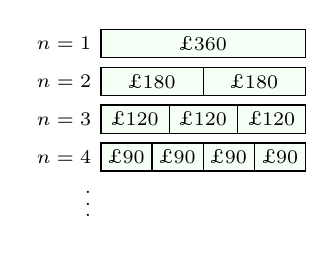
\begin{tikzpicture}[baseline=(current bounding box.center)]
  \foreach \p/\y in {1/0,2/-0.48,3/-0.96,4/-1.44} {
    \node[font=\scriptsize,left] at (0,\y+0.18) {$n=\p$};
    \begin{scope}[shift={(0,\y)}]\sharebar{\p}\end{scope}}
  \node[font=\scriptsize,left] at (0,-1.75) {$\vdots$};
  \end{tikzpicture}}

% A pizza cut into n equal slices, with the angle of one slice marked.
\newcommand{\pizza}[1]{\pic{%
  \pgfmathtruncatemacro{\ang}{360/#1}
  \draw[fill=yellow!10,line width=0.6pt] (0,0) circle (0.5);
  \ifnum#1>1
    \foreach \k in {1,...,#1} {\draw (0,0) -- ({90+360*\k/#1}:0.5);}
    \draw[line width=0.4pt] (90:0.13) arc (90:{90+360/#1}:0.13);
    \node[font=\tiny,inner sep=0pt] at ({90+180/#1}:0.3) {$\ang^\circ$};
  \else
    \node[font=\tiny,inner sep=0pt] at (0,0) {$\ang^\circ$};
  \fi}}

% Pattern n of the garden path: a row of n grey slabs with a border of
% white slabs, so 3 rows of n+2 slabs.
\newcommand{\gardenpath}[1]{\pic{%
  \pgfmathtruncatemacro{\w}{#1+2}
  \draw[black!70,line width=0.4pt,step=0.28] (0,0) grid ({0.28*\w},0.84);
  \foreach \c in {1,...,#1} {\filldraw[fill=gray!55,draw=black!70,line width=0.4pt]
    ({0.28*\c},0.28) rectangle ++(0.28,0.28);}}}

% Pattern n of the fraction bars: a bar cut into 2n+1 equal parts, with
% 2n-1 parts shaded. Every bar is the same length.
\newcommand{\fracbar}[1]{%
  \pgfmathtruncatemacro{\parts}{2*#1+1}
  \pgfmathtruncatemacro{\shaded}{2*#1-1}
  \foreach \k in {1,...,\parts} {
    \ifnum\k>\shaded\relax \def\barfill{white}\else \def\barfill{gray!40}\fi
    \draw[fill=\barfill,line width=0.5pt] ({2.8*(\k-1)/\parts},0) rectangle ({2.8*\k/\parts},0.3);}}

% The table for a picture sequence, with one \picrow for each row. The
% last column holds the nth term.
\newenvironment{pictable}{%
  \setlength{\tabcolsep}{2pt}%
  \begin{tabular}{|C{1.85cm}|*{6}{C{0.74cm}|}C{1.75cm}|}\hline
  {\small Pattern $n$} & 1 & 2 & 3 & 4 & 5 & 10 & {\small $n$th term}\\\hline}
  {\end{tabular}}
\newcommand{\picrow}[1]{{\small #1} & & & & & & & \rowstrut\\\hline}

% ----------------------------------------------------------------
% Part 4. A stack of n cups, drawn 1 cm to 0.1 cm. Each cup is 11 cm
% tall, and each cup added raises the top of the stack by 2 cm, so the
% stack is 2n+9 cm tall. The cups are drawn from the top of the stack
% down, so that each cup hides the part of the cup above it that sits
% inside it.
\newcommand{\cupstack}[1]{%
  \foreach \k in {#1,...,1} {
    \pgfmathsetmacro{\y}{0.2*(\k-1)}
    \draw[fill=white,line width=0.5pt] (-0.27,\y) -- (0.27,\y) -- (0.41,\y+1.1) -- (-0.41,\y+1.1) -- cycle;
    \draw[line width=1.1pt,line cap=round] (-0.44,\y+1.1) -- (0.44,\y+1.1);}}
% A stack of n chairs seen from the side, drawn 1 cm to 0.016 cm. Each
% chair is 85 cm tall, and each chair added raises the stack by 10 cm,
% so the stack is 10n+75 cm tall.
\newcommand{\chairstack}[1]{%
  \foreach \k in {1,...,#1} {
    \pgfmathsetmacro{\y}{0.16*(\k-1)}
    \draw[line width=0.7pt,line cap=round,line join=round]
      (0,\y) -- (0.08,\y+0.72) -- (0.86,\y+0.72) -- (0.94,\y)
      (0.08,\y+0.72) -- (0.02,\y+1.36);}}
% The height of a stack, marked beside it: \stackheight{<x>}{<top>}{<label>}
\newcommand{\stackheight}[3]{%
  \draw[dim] (#1,0) -- (#1,#2) node[midway,left,font=\scriptsize,inner sep=2pt] {#3};}

% Characters this language's font has not got are borrowed from another,
% rather than being silently dropped - see docs/translated-sheet-latex.md
\directlua{%
  if luaotfload and luaotfload.add_fallback then
    luaotfload.add_fallback("eallatinfallback",
      { "Noto Serif:mode=harf;" })
  else
    tex.error("this luaotfload is too old to register a fallback font")
  end
}
\usepackage[english]{babel}
\babelprovide[import]{polish}
\babelfont[polish]{rm}[Renderer=Harfbuzz, BoldFont={Noto Serif}, ItalicFont={Noto Serif}, BoldItalicFont={Noto Serif}, RawFeature={fallback=eallatinfallback}]{Noto Serif}
\babelfont[polish]{sf}[Renderer=Harfbuzz, BoldFont={Noto Serif}, ItalicFont={Noto Serif}, BoldItalicFont={Noto Serif}, RawFeature={fallback=eallatinfallback}]{Noto Serif}
\newcommand{\ealtext}[1]{\foreignlanguage{polish}{#1}}
\newcommand{\ealtextblock}[1]{{\raggedright\foreignlanguage{polish}{#1}\par}}
% ================================================================
% EAL layout helpers
% ================================================================
\usepackage{xcolor}

\definecolor{ealkeycolour}{RGB}{0,128,0}
\definecolor{ealenglish}{RGB}{0,0,0}
\definecolor{ealtwocolour}{RGB}{112,48,160}

\newsavebox{\ealboxen}
\newsavebox{\ealboxtr}
\newlength{\ealglosswd}
\newlength{\ealglossraise}
\setlength{\ealglossraise}{1.15em}

% a tier 3 word, in English and in translation alike
\newcommand{\ealkey}[1]{\textcolor{ealkeycolour}{#1}}
\newcommand{\ealkeytr}[1]{\textcolor{ealkeycolour}{\ealtext{#1}}}

% One translated word above one English word. Built from kernel
% primitives, never a tabular, which would break wherever the sheet
% loads array, booktabs or tabularx. The box is as wide as the wider of
% the two, so a long translation pushes its neighbours aside instead of
% overlapping them, and it claims its full height so a table row or a
% TikZ node makes room for it.
\newcommand{\ealgloss}[2]{%
  \sbox{\ealboxen}{\ealkey{#1}}%
  \sbox{\ealboxtr}{\small\textcolor{ealtwocolour}{\ealtext{#2}}}%
  \setlength{\ealglosswd}{\wd\ealboxen}%
  \ifdim\wd\ealboxtr>\ealglosswd\setlength{\ealglosswd}{\wd\ealboxtr}\fi
  \leavevmode
  \makebox[\ealglosswd][c]{%
    \makebox[0pt][c]{\usebox{\ealboxen}}%
    \makebox[0pt][c]{\raisebox{\ealglossraise}{\usebox{\ealboxtr}}}%
  }%
}

% opens up line spacing around a block of glosses, so the raised
% translations sit clear of the line above
\newenvironment{ealglossed}{\par\linespread{2.1}\selectfont\ignorespaces}{\par}

% a whole translated sentence above its English counterpart. block level,
% so it does not belong inside a tabular cell
\newcommand{\ealpara}[2]{%
  \par\addvspace{0.5\baselineskip}%
  {\color{ealtwocolour}\ealtextblock{#1}}%
  \penalty200
  {\color{ealenglish}#2\par}%
  \addvspace{0.5\baselineskip}%
}

\begin{document}

\begin{center}
  {\Large\bfseries Sequences and Equations}\\[1pt]
  {\small Extension}
\end{center}
\vspace{-10pt}

% ================================================================
\ealpara{Kiedy dwa \ealkeytr{ciągi} się spotykają?}{When do two \ealkey{sequences} meet?}
\parttitle{1}{When do two sequences meet?}

\begin{keyidea}
\ealpara{Dwa \ealkeytr{ciągi} mają równe \ealkeytr{wyrazy} na tej samej \ealkeytr{pozycji}, gdy ich \ealkeytr{wzory na $n$-ty wyraz} są równe.}{Two \ealkey{sequences} have \textbf{equal \ealkey{terms} in the same \ealkey{position}} when their \ealkey{$n$th terms} are equal.}

\ealpara{Zapisujemy jeden \ealkeytr{wzór na $n$-ty wyraz} jako równy drugiemu i \ealkeytr{rozwiązujemy} \ealkeytr{równanie}, wykonując tę samą czynność po obu stronach.}{We write one \ealkey{$n$th term} equal to the other, and \ealkey{solve} the \ealkey{equation} by doing the same thing to both sides.}

\ealpara{\ealkeytr{Rozwiązanie} $n$ jest \ealkeytr{pozycją}, więc musi być \ealkeytr{liczbą dodatnią} i \ealkeytr{liczbą całkowitą nieujemną}.}{The \ealkey{solution} $n$ is a \ealkey{position}, so it must be a \ealkey{positive} \ealkey{whole number}.}

\ealpara{Jeśli tak nie jest, \ealkeytr{ciągi} nigdy nie mają równych \ealkeytr{wyrazów} na tej samej \ealkeytr{pozycji}.}{If it is not, the \ealkey{sequences} never have equal \ealkey{terms} in the same \ealkey{position}.}
\end{keyidea}

\begin{wex}{the sequences $5n+3$ and $3n+17$}
\meetlayout
  {\termtable[1 & 2 & 3 & 4 & 5 & 6 & \hl{7} & 8]
    {$5n+3$}{8 & 13 & 18 & 23 & 28 & 33 & \hl{38} & 43}
    {$3n+17$}{20 & 23 & 26 & 29 & 32 & 35 & \hl{38} & 41}}
  {\begin{working}
     5n+3 & = & 3n+17\\ \bsop{-3n}
     2n+3 & = & 17\\ \bsop{-3}
     2n & = & 14\\ \bsop{\div 2}
     n & = & 7
   \end{working}}
  {\ealpara{Wyrazy na \ealkeytr{pozycji} \textbf{7} są równe.}{The \ealkey{terms} in \ealkey{position} \textbf{7} are equal.}\par\smallskip
   \ealpara{Sprawdzenie: $5\times7+3=38$ i $3\times7+17=38$.}{Check: $5\times7+3=38$ and $3\times7+17=38$.}}
\end{wex}

\begin{enumerate}
\item \ealpara{Użyj tej samej metody, aby znaleźć, kiedy \ealkeytr{ciągi} $7n+2$ i $4n+26$ mają równe \ealkeytr{wyrazy}.}{Use the same method to find when the \ealkey{sequences} $7n+2$ and $4n+26$ have equal \ealkey{terms}.}\par
\meetlayout
  {\termtable{$7n+2$}{9 & & & & & & &}{$4n+26$}{30 & & & & & & &}}
  {\begin{working}
     7n+2 & = & 4n+26\\ \bsop{-4n}
     \sidegap & = & \sidegap\\ \bsop{-2}
     \sidegap & = & \sidegap\\ \bsop{\div 3}
     n & = & \sidegap
   \end{working}}
  {\ealpara{Wyrazy na \ealkeytr{pozycji} \gap\ są równe.}{The \ealkey{terms} in \ealkey{position} \gap\ are equal.}\par\smallskip
   \ealpara{Sprawdzenie: \ansline[3.4cm] i \ansline[3.4cm].}{Check: \ansline[3.4cm] and \ansline[3.4cm].}}

\item \ealpara{Znajdź, kiedy \ealkeytr{ciągi} $9n-4$ i $5n+20$ mają równe \ealkeytr{wyrazy}.}{Find when the \ealkey{sequences} $9n-4$ and $5n+20$ have equal \ealkey{terms}.}\par
\meetlayout
  {\termtable{$9n-4$}{ & & & & & & &}{$5n+20$}{ & & & & & & &}}
  {\begin{working}
     9n-4 & = & 5n+20\\ \bsopgap
     \sidegap & = & \sidegap\\ \bsopgap
     \sidegap & = & \sidegap\\ \bsopgap
     n & = & \sidegap
   \end{working}}
  {\ealpara{Wyrazy na \ealkeytr{pozycji} \gap\ są równe.}{The \ealkey{terms} in \ealkey{position} \gap\ are equal.}\par\smallskip
   \ealpara{Sprawdzenie: \ansline[3.4cm] i \ansline[3.4cm].}{Check: \ansline[3.4cm] and \ansline[3.4cm].}}

\item \begin{minipage}[t]{0.5\linewidth}
  \ealpara{Dwie świece są zapalone w tym samym czasie.}{Two candles are lit at the same time.}
  \ealpara{Świeca A ma 30\,cm wysokości i skraca się o 2\,cm każdą godzinę.}{Candle A is 30\,cm tall and burns down by 2\,cm every hour.}
  \ealpara{Świeca B ma 21\,cm wysokości i skraca się o 1\,cm każdą godzinę.}{Candle B is 21\,cm tall and burns down by 1\,cm every hour.}
  \begin{enumerate}
  \item \ealpara{Zapisz \ealkeytr{wyrażenie} na wysokość każdej świecy po $n$ godzinach.}{Write an \ealkey{expression} for the height of each candle after $n$ hours.}\par
    A: \ansline[2.4cm] \quad B: \ansline[2.4cm]
  \end{enumerate}
  \end{minipage}\hfill
  \begin{minipage}[t]{0.47\linewidth}\raggedleft\vspace{0pt}
  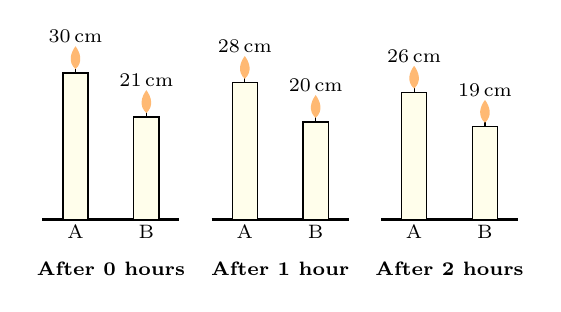
\begin{tikzpicture}[baseline=(current bounding box.north)]
    \candlepair{0}{0 hours}{30}{21}
    \candlepair{2.15}{1 hour}{28}{20}
    \candlepair{4.3}{2 hours}{26}{19}
  \end{tikzpicture}\end{minipage}
  \begin{enumerate}[start=2]
  \item \ealpara{\ealkeytr{Rozwiąż} \ealkeytr{równanie}, aby znaleźć, kiedy dwie świece są tej samej wysokości. Jakie są wtedy wysokie?}{\ealkey{Solve} an \ealkey{equation} to find when the two candles are the same height. How tall are they then?}
    \workspace{1.6cm}
  \item \ealpara{Która świeca wypali się pierwsza? Wyjaśnij, skąd to wiesz.}{Which candle burns out first? Explain how you know.}\par\vspace{9pt}\hrulefill
  \end{enumerate}

% (a) Ella: 100-3n, Finn: 64+6n. (b) 100-3n = 64+6n gives 36 = 9n,
% n = 4, when both are at 88%.
\newpage
\item \begin{minipage}[t]{0.52\linewidth}
  \ealpara{Telefon Elli jest naładowany w 100\% i traci 3\% naładowania każdą godzinę.}{Ella's phone is 100\% charged and loses 3\% of its charge every hour.}
  \ealpara{Telefon Finna jest naładowany w 64\% i się ładuje, więc zyskuje 6\% każdą godzinę.}{Finn's phone is 64\% charged and is charging, so it gains 6\% every hour.}
  \begin{enumerate}
  \item \ealpara{Zapisz \ealkeytr{wyrażenie} na poziom naładowania każdego telefonu po $n$ godzinach.}{Write an \ealkey{expression} for the charge of each phone after $n$ hours.}\par
    Ella: \ansline[2.2cm] \quad Finn: \ansline[2.2cm]
  \item \ealpara{Po ilu godzinach dwa telefony mają takie samo naładowanie?}{After how many hours do the two phones have the same charge?}
  \end{enumerate}
  \end{minipage}\hfill
  \begin{minipage}[t]{0.45\linewidth}\raggedleft\vspace{0pt}
  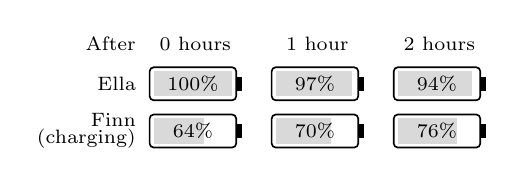
\begin{tikzpicture}[baseline=(current bounding box.north)]
    \foreach \h/\x in {0 hours/0,1 hour/1.55,2 hours/3.1} {
      \node[font=\scriptsize] at (\x+0.58,0.72) {\h};}
    \node[font=\scriptsize,left] at (-0.05,0.72) {After};
    \node[font=\scriptsize,left] at (-0.05,0.21) {Ella};
    \node[font=\scriptsize,left,align=right] at (-0.05,-0.39) {Finn\\[-2pt](charging)};
    \battery{0}{0}{100}\battery{1.55}{0}{97}\battery{3.1}{0}{94}
    \battery{0}{-0.6}{64}\battery{1.55}{-0.6}{70}\battery{3.1}{-0.6}{76}
  \end{tikzpicture}\end{minipage}
  \workspace{2.6cm}

% (a) 2n = 7, n = 3.5, which is not a whole number. (b) Both go up by 6
% each time, and 6n+5 is always 4 more than 6n+1. (c) 2n = c-1, so
% c = 3, 5, 7, ... Every possible c is an odd number of at least 3.
\item
  \begin{enumerate}
  \item \ealpara{\ealkeytr{Rozwiąż} \ealkeytr{równanie}, aby pokazać, że \ealkeytr{ciągi} $4n+1$ i $2n+8$ nigdy nie mają równych \ealkeytr{wyrazów} na tej samej \ealkeytr{pozycji}.}{\ealkey{Solve} an \ealkey{equation} to show that the \ealkey{sequences} $4n+1$ and $2n+8$ never have equal \ealkey{terms} in the same \ealkey{position}.}\par\vspace{2.5cm}
  \item \ealpara{Bez \ealkeytr{rozwiązywania} \ealkeytr{równania} wyjaśnij, dlaczego $6n+1$ i $6n+5$ nigdy nie mają równych \ealkeytr{wyrazów} na tej samej \ealkeytr{pozycji}.}{Without \ealkey{solving} an \ealkey{equation}, explain why $6n+1$ and $6n+5$ never have equal \ealkey{terms} in the same \ealkey{position}.} \hrulefill\par\vspace{9pt}\hrulefill
  \item \ealpara{\ealkeytr{Ciągi} $4n+1$ i $2n+c$ mają równe \ealkeytr{wyrazy} na tej samej \ealkeytr{pozycji}, gdzie $c$ jest \ealkeytr{liczbą całkowitą nieujemną}. Znajdź trzy możliwe wartości $c$. Co mają wspólnego wszystkie możliwe wartości $c$?}{The \ealkey{sequences} $4n+1$ and $2n+c$ do have equal \ealkey{terms} in the same \ealkey{position}, where $c$ is a \ealkey{whole number}. Find three possible values of $c$. What do all the possible values of $c$ have in common?}\par\vspace{6pt}
    \ealpara{$c=$ \gap, \gap\ lub \gap}{$c=$ \gap, \gap\ or \gap \qquad \hrulefill}
  \end{enumerate}
\end{enumerate}

% ================================================================
\ealpara{Porównywanie \ealkeytr{wyrazów} na różnych \ealkeytr{pozycjach}}{Comparing \ealkey{terms} in different \ealkey{positions}}
\parttitle{2}{Comparing terms in different positions}

\begin{keyidea}
\ealpara{Aby zapisać \ealkeytr{wyraz} na \ealkeytr{pozycji} $n+4$ \ealkeytr{ciągu} $3n+1$, zastępujemy $n$ przez $n+4$, otrzymując $3(n+4)+1$.}{To write the \ealkey{term} in \ealkey{position} $n+4$ of the \ealkey{sequence} $3n+1$, we replace $n$ with $n+4$ to get $3(n+4)+1$.}

\ealpara{\ealkeytr{Nawiasy} pokazują, że całe $n+4$ jest pomnożone przez 3.}{The \ealkey{brackets} show that all of $n+4$ is multiplied by 3.}

\ealpara{Najpierw \ealkeytr{wymnażamy} \ealkeytr{nawiasy} (pamiętaj: $3(n+4)=3\times n+3\times4=3n+12$), a następnie \ealkeytr{rozwiązujemy} \ealkeytr{równanie}, wykonując tę samą czynność po obu stronach.}{We \ealkey{expand} the \ealkey{brackets} first (remember $3(n+4)=3\times n+3\times4=3n+12$), and then \ealkey{solve} the \ealkey{equation} by doing the same thing to both sides.}
\end{keyidea}

\begin{wex}{houses and squares}
\ealpara{Sam układa rząd domków z zapałek.}{Sam makes a row of houses from matchsticks.}
\ealpara{Jo układa rząd kwadratów, o 4 więcej kwadratów niż Sam ma domków.}{Jo makes a row of squares, with 4 more squares than Sam has houses.}
\ealpara{Używają tej samej liczby zapałek.}{They use the same number of matchsticks.}
\ealpara{Ile domków układa Sam?}{How many houses does Sam make?}\par\smallskip
\begin{minipage}[t]{0.49\linewidth}\centering
  \threepatterns{\chainhouses{1}}{\chainhouses{2}}{\chainhouses{3}}\par
  {\small \ealpara{Wzór $n$ ma $n$ domków i $5n+1$ zapałek.}{\ealkey{Pattern} $n$ has $n$ houses and $5n+1$ matchsticks.}}
\end{minipage}\hfill
\begin{minipage}[t]{0.49\linewidth}\centering
  \threepatterns{\chainsquares{1}}{\chainsquares{2}}{\chainsquares{3}}\par
  {\small \ealpara{Wzór $n$ ma $n$ kwadratów i $3n+1$ zapałek.}{\ealkey{Pattern} $n$ has $n$ squares and $3n+1$ matchsticks.}}
\end{minipage}\par\medskip
\ealpara{\ealkeytr{Wymnażać} \ealkeytr{nawiasy}}{\ealkey{expand} the \ealkey{brackets}}
\eqlayout{0.6}
  {\ealpara{Sam układa $n$ domków, które zużywają $5n+1$ zapałek.}{Sam makes $n$ houses, which use $5n+1$ matchsticks.}\par\smallskip
   \ealpara{Jo układa $n+4$ kwadratów, które zużywają $3(n+4)+1$ zapałek.}{Jo makes $n+4$ squares, which use $3(n+4)+1$ matchsticks.}\par\smallskip
   \ealpara{Liczby zapałek są równe, więc zapisujemy jedną równą drugiej.}{The numbers of matchsticks are equal, so we write one equal to the other.}}
  {\begin{working}
     5n+1 & = & 3(n+4)+1\\ \bsnote{\ealkey{expand} the \ealkey{brackets}}
     5n+1 & = & 3n+13\\ \bsop{-3n}
     2n+1 & = & 13\\ \bsop{-1}
     2n & = & 12\\ \bsop{\div 2}
     n & = & 6
   \end{working}}
  {\ealpara{Sam układa \textbf{6} domków, a Jo układa \textbf{10} kwadratów.}{Sam makes \textbf{6} houses and Jo makes \textbf{10} squares.}
   \ealpara{Sprawdzenie: $5\times6+1=31$ i $3\times10+1=31$.}{Check: $5\times6+1=31$ and $3\times10+1=31$.}}
\end{wex}

\begin{enumerate}[resume]
\newpage
% (a) The difference between each pair of terms is the same. (b)
% x+2 = 2x-4, x = 6. (c) 7, 15, 23; 8n-1.
\item \ealpara{Pierwsze trzy \ealkeytr{wyrazy} \ealkeytr{ciągu liniowego} to $x+1$, $2x+3$ i $4x-1$.}{The first three \ealkey{terms} of a \ealkey{linear} \ealkey{sequence} are $x+1$, $2x+3$ and $4x-1$.}
\begin{enumerate}
\item \ealpara{Wyjaśnij, dlaczego $(2x+3)-(x+1)=(4x-1)-(2x+3)$.}{Explain why $(2x+3)-(x+1)=(4x-1)-(2x+3)$.} \hrulefill
\item \ealpara{\ealkeytr{Rozwiąż} \ealkeytr{równanie}, aby znaleźć $x$. Następnie zapisz pierwsze trzy \ealkeytr{wyrazy} i \ealkeytr{wzór na $n$-ty wyraz} \ealkeytr{ciągu}.}{\ealkey{Solve} the \ealkey{equation} to find $x$. Then write the first three \ealkey{terms} and the \ealkey{$n$th term} of the \ealkey{sequence}.}
  \workspace{1.8cm}
\end{enumerate}

% Triangles: 2n+1. 5n+1 = 2(n+12)+1, 5n+1 = 2n+25, 3n+1 = 25, 3n = 24,
% n = 8. Ali makes 8 houses and Bea makes 20 triangles: 41 matchsticks.
\item \ealpara{Ali układa rząd domków.}{Ali makes a row of houses.}
\ealpara{Bea układa rząd trójkątów, o 12 więcej trójkątów niż Ali ma domków.}{Bea makes a row of triangles, with 12 more triangles than Ali has houses.}
\ealpara{Używają tej samej liczby zapałek.}{They use the same number of matchsticks.}
\ealpara{Ile domków układa Ali?}{How many houses does Ali make?}\par\smallskip
\begin{minipage}[t]{0.49\linewidth}\centering
  \threepatterns{\chainhouses{1}}{\chainhouses{2}}{\chainhouses{3}}\par
  {\small \ealpara{Wzór $n$ ma $n$ domków i $5n+1$ zapałek.}{\ealkey{Pattern} $n$ has $n$ houses and $5n+1$ matchsticks.}}
\end{minipage}\hfill
\begin{minipage}[t]{0.49\linewidth}\centering
  \threepatterns{\chaintriangles{1}}{\chaintriangles{2}}{\chaintriangles{3}}\par
  {\small \ealpara{Wzór $n$ ma $n$ trójkątów i \ansline[1.4cm] zapałek.}{\ealkey{Pattern} $n$ has $n$ triangles and \ansline[1.4cm] matchsticks.}}
\end{minipage}\par\medskip
\ealpara{\ealkeytr{Wymnażać} \ealkeytr{nawiasy}}{\ealkey{expand} the \ealkey{brackets}}
\eqlayout{0.6}
  {\ealpara{Ali układa $n$ domków, które zużywają $5n+1$ zapałek.}{Ali makes $n$ houses, which use $5n+1$ matchsticks.}\par\smallskip
   \ealpara{Bea układa \ansline[1.1cm] trójkątów, które zużywają \ansline[1.9cm] zapałek.}{Bea makes \ansline[1.1cm] triangles, which use \ansline[1.9cm] matchsticks.}\par\smallskip
   \ealpara{Liczby zapałek są równe, więc zapisujemy jedną równą drugiej.}{The numbers of matchsticks are equal, so we write one equal to the other.}}
  {\begin{working}
     \sidegap & = & \sidegap[2.2cm]\\ \bsnote{\ealkey{expand} the \ealkey{brackets}}
     \sidegap & = & \sidegap\\ \bsop{-2n}
     \sidegap & = & \sidegap\\ \bsop{-1}
     \sidegap & = & \sidegap\\ \bsop{\div 3}
     n & = & \sidegap
   \end{working}}
  {\ealpara{Ali układa \gap\ domków, a Bea układa \gap\ trójkątów.}{Ali makes \gap\ houses and Bea makes \gap\ triangles.}
   \ealpara{Sprawdzenie: \ansline[2.9cm] i \ansline[2.9cm].}{Check: \ansline[2.9cm] and \ansline[2.9cm].}}

% (a) n panels and n+1 posts. (b) 25n+8(n+1) = 338, 33n+8 = 338,
% 33n = 330, n = 10. (c) 31n+4(n+1) = 25n+8(n+1), 35n+4 = 33n+8,
% n = 2. For 10 panels A costs 338 pounds and B costs 354 pounds, so A
% is cheaper.
\item \begin{minipage}[t]{0.6\linewidth}
  \ealpara{Płot ma słupek na każdym końcu i słupek między każdą parą paneli.}{A fence has a post at each end and a post between each pair of panels.}
  \ealpara{W centrum ogrodniczym A panel kosztuje \pounds25, a słupek kosztuje \pounds8.}{At garden centre A, a panel costs \pounds25 and a post costs \pounds8.}
  \end{minipage}\hfill
  \begin{minipage}[t]{0.37\linewidth}\raggedleft\vspace{0pt}
  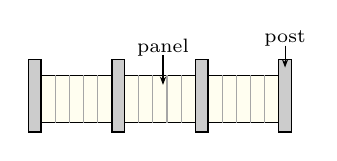
\begin{tikzpicture}[baseline=(current bounding box.north)]
    \fence{3}
    \node[lab,above] at (1.71,0.92) {panel};
    \draw[-{Stealth[length=3pt]},line width=0.4pt] (1.71,0.98) -- (1.71,0.6);
    \node[lab,above] at (3.26,1.05) {post};
    \draw[-{Stealth[length=3pt]},line width=0.4pt] (3.26,1.1) -- (3.26,0.82);
  \end{tikzpicture}\end{minipage}
  \begin{enumerate}
  \item \ealpara{Wyjaśnij, dlaczego płot z $n$ paneli kosztuje $25n+8(n+1)$ funtów w centrum ogrodniczym A.}{Explain why a fence of $n$ panels costs $25n+8(n+1)$ pounds at garden centre A.}
    \par\vspace{9pt}\hrulefill
  \item \ealpara{Płot z centrum ogrodniczego A kosztuje \pounds338. Ile ma paneli?}{A fence from garden centre A costs \pounds338. How many panels does it have?}
    \workspace{1.1cm}
  \item \ealpara{W centrum ogrodniczym B panel kosztuje \pounds31, a słupek kosztuje \pounds4.}{At garden centre B, a panel costs \pounds31 and a post costs \pounds4.}
    \ealpara{Przy ilu panelach oba centra ogrodnicze pobierają tę samą opłatę?}{For how many panels do the two garden centres charge the same?}
    \ealpara{Które centrum ogrodnicze jest tańsze dla płotu z 10 paneli?}{Which garden centre is cheaper for a fence of 10 panels?}
    \workspace{1.4cm}
  \end{enumerate}

% (a) 9x-20 and 27x-65. (b) 27x-65 = 205, 27x = 270, x = 10.
\item \ealpara{Naukowiec hoduje komórki w naczyniu.}{A scientist grows cells in a dish.}
\ealpara{Co godzinę liczba komórek się potraja, a następnie 5 komórek jest pobieranych do badania.}{Every hour the number of cells triples, and then 5 cells are taken out to be tested.}
\ealpara{Na początku jest $x$ komórek.}{There are $x$ cells at the start.}\par
\begin{minipage}[t]{0.5\linewidth}
  \begin{enumerate}
  \item \ealpara{Uzupełnij tabelę.}{Complete the table.}
    \ealpara{\ealkeytr{Wymnażaj} \ealkeytr{nawiasy} w każdym \ealkeytr{wyrazie}.}{\ealkey{Expand} the \ealkey{brackets} in each \ealkey{term}.}
  \item \ealpara{Po 3 godzinach jest 205 komórek. Ile komórek było na początku?}{After 3 hours there are 205 cells. How many cells were there at the start?}
  \end{enumerate}
\end{minipage}\hfill
\begin{minipage}[t]{0.47\linewidth}\raggedleft\vspace{0pt}
  {\setlength{\tabcolsep}{3pt}\renewcommand{\arraystretch}{1.3}%
  \begin{tabular}{|l|C{0.55cm}|C{1.2cm}|C{2.3cm}|C{1.5cm}|}\hline
  {\small Hours} & 0 & 1 & 2 & 3\\\hline
  {\small Cells}\rowstrut & $x$ & $3x-5$ & $3(3x-5)-5$\newline${}=$\ansline[1.3cm] & \\\hline
  \end{tabular}}
\end{minipage}
\workspace{1.6cm}
\end{enumerate}

% ================================================================
\newpage
\ealpara{\ealkeytr{Niewiadoma} w \ealkeytr{mianowniku}}{The \ealkey{unknown} in the \ealkey{denominator}}
\parttitle{3}{The unknown in the denominator}

\begin{keyidea}
\ealpara{W niektórych \ealkeytr{ciągach} \ealkeytr{pozycja} $n$ jest w \ealkeytr{mianowniku} \ealkeytr{ułamka}, na przykład $\frac{360}{n}$.}{In some \ealkey{sequences} the \ealkey{position} $n$ is in the \ealkey{denominator} of a \ealkey{fraction}, such as $\frac{360}{n}$.}

\ealpara{Aby \ealkeytr{rozwiązać} \ealkeytr{równanie} z $n$ w \ealkeytr{mianowniku}, mnożymy obie strony przez \ealkeytr{mianownik} (pamiętaj: $\frac{360}{n}\times n=360$).}{To \ealkey{solve} an \ealkey{equation} with $n$ in the \ealkey{denominator}, we multiply both sides by the \ealkey{denominator} (remember $\frac{360}{n}\times n=360$).}

\ealpara{To daje \ealkeytr{równanie} bez \ealkeytr{ułamków}, które \ealkeytr{rozwiązujemy}, wykonując tę samą czynność po obu stronach.}{This gives an \ealkey{equation} with no \ealkey{fractions}, which we \ealkey{solve} by doing the same thing to both sides.}
\end{keyidea}

\begin{wex}{sharing the cost of a minibus}
\ealpara{Wynajem minibusa na wycieczkę dzienną kosztuje \pounds360.}{A minibus costs \pounds360 to hire for a day trip.}
\ealpara{Koszt jest dzielony po równo między $n$ osób, które jadą, więc każda osoba płaci $\frac{360}{n}$ funtów.}{The cost is shared equally between the $n$ people who go, so each person pays $\frac{360}{n}$ pounds.}
\ealpara{Ile osób musi pojechać, aby koszt wyniósł \pounds24 na osobę?}{How many people must go for the cost to be \pounds24 each?}\par\smallskip
\eqlayout{0.55}
  {\centering\sharebars}
  {\begin{working}
     \dfrac{360}{n} & = & 24\\[4pt] \bsop{\times n}
     360 & = & 24n\\ \bsop{\div 24}
     15 & = & n
   \end{working}}
  {\ealpara{Musi pojechać \textbf{15} osób.}{\textbf{15} people must go.}
   \ealpara{Sprawdzenie: $360\div15=24$.}{Check: $360\div15=24$.}}
\end{wex}

\begin{enumerate}[resume]
% 360/n = 40, 360 = 40n, 9 = n. (b) 360/n = 25 gives n = 14.4, which is
% not a whole number, so no.
\item \ealpara{Pizzę kroi się na $n$ równych kawałków, więc \ealkeytr{kąt} każdego kawałka wynosi $\frac{360}{n}$ \ealkeytr{stopni}.}{A pizza is cut into $n$ equal slices, so the \ealkey{angle} of each slice is $\frac{360}{n}$ \ealkey{degrees}.}
\ealpara{Na ile kawałków trzeba pokroić pizzę, aby każdy \ealkeytr{kąt} wynosił $40^\circ$?}{How many slices must the pizza be cut into for each \ealkey{angle} to be $40^\circ$?}\par\smallskip
\eqlayout{0.55}
  {\centering\threepatterns{\pizza{1}}{\pizza{2}}{\pizza{3}}\hspace{10pt}%
   \begin{tabular}[b]{@{}c@{}}\pizza{4}\\[-1pt]{\scriptsize Pattern 4}\end{tabular}}
  {\begin{working}
     \dfrac{360}{n} & = & 40\\[4pt] \bsop{\times n}
     \sidegap & = & \sidegap\\ \bsop{\div 40}
     \sidegap & = & n
   \end{working}}
  {\ealpara{\gap\ kawałków.}{\gap\ slices.}
   \ealpara{Sprawdzenie: \ansline[3.4cm].}{Check: \ansline[3.4cm].}}\par\medskip
\ealpara{Czy pizzę można pokroić na równe kawałki o \ealkeytr{kącie} $25^\circ$?}{Can a pizza be cut into equal slices with an \ealkey{angle} of $25^\circ$?}
\ealpara{\ealkeytr{Rozwiąż} \ealkeytr{równanie}, aby to wyjaśnić.}{\ealkey{Solve} an \ealkey{equation} to explain.}\par\vspace{1.6cm}\hrulefill

% (a) Grey: 1,2,3,4,5,10; n. Total: 9,12,15,18,21,36; 3n+6.
% (b) n/(3n+6). (c) 10n = 3(3n+6), 10n = 9n+18, n = 18 (18/60 = 3/10).
% (d) 3n = 3n+6 gives 0 = 6, which is never true. There are 2n+6 white
% slabs, which is always more than twice the n grey slabs.
\item \ealpara{Ścieżka ogrodowa jest zrobiona z rzędu szarych płyt z obramowaniem z białych płyt.}{A garden path is made from a row of grey slabs with a border of white slabs.}
\begin{enumerate}
\item \ealpara{Uzupełnij tabelę i zapisz \ealkeytr{wzór na $n$-ty wyraz}.}{Complete the table and write each \ealkey{$n$th term}.}\par
  \begin{minipage}[c]{0.4\linewidth}
  \threepatterns{\gardenpath{1}}{\gardenpath{2}}{\gardenpath{3}}
  \end{minipage}\hfill
  \begin{minipage}[c]{0.59\linewidth}\raggedleft
  \begin{pictable}\picrow{Grey slabs}\picrow{All slabs}\end{pictable}
  \end{minipage}
\item \ealpara{Zapisz \ealkeytr{ułamek} płyt w \ealkeytr{wzorze} $n$, które są szare. \ansline[2.5cm]}{Write the \ealkey{fraction} of the slabs in \ealkey{pattern} $n$ that are grey. \ansline[2.5cm]}
\item \ealpara{Który \ealkeytr{wzór} ma dokładnie $\frac{3}{10}$ szarych płyt?}{Which \ealkey{pattern} has exactly $\frac{3}{10}$ of its slabs grey?}
  \ealpara{Pomnóż obie strony swojego \ealkeytr{równania} przez 10 i przez \ealkeytr{mianownik}.}{Multiply both sides of your \ealkey{equation} by 10 and by the \ealkey{denominator}.}
  \workspace{1.9cm}
\item \ealpara{Pokaż, że żaden \ealkeytr{wzór} nie ma dokładnie $\frac{1}{3}$ szarych płyt.}{Show that no \ealkey{pattern} has exactly $\frac{1}{3}$ of its slabs grey.}
  \ealpara{Użyj rysunku, aby wyjaśnić dlaczego.}{Use the picture to explain why.}
  \vspace{1.5cm}\par\hrulefill
\end{enumerate}

% (a) (2n-1)/(2n+1). (b) 2n-1 = 0.92(2n+1), 0.16n = 1.92, n = 12, which
% is 23/25. (c) 2n-1 = 0.95(2n+1), 0.1n = 1.95, n = 19.5, so no.
% (d) It gets closer to 1, but there are always 2 parts not shaded.
\newpage
\item \begin{minipage}[t]{0.56\linewidth}
  \ealpara{\ealkeytr{Wzór} $n$ tego \ealkeytr{ciągu} to pasek podzielony na $2n+1$ równych części, z których $2n-1$ jest \ealkeytr{zacieniowanych}.}{\ealkey{Pattern} $n$ of this \ealkey{sequence} is a bar cut into $2n+1$ equal parts, with $2n-1$ of the parts \ealkey{shaded}.}
  \begin{enumerate}
  \item \ealpara{Zapisz \ealkeytr{ułamek} paska, który jest \ealkeytr{zacieniowany} we \ealkeytr{wzorze} $n$. \ansline[1.6cm]}{Write the \ealkey{fraction} of the bar that is \ealkey{shaded} in \ealkey{pattern} $n$. \ansline[1.6cm]}
  \end{enumerate}
  \end{minipage}\hfill
  \begin{minipage}[t]{0.42\linewidth}\raggedleft\vspace{0pt}
  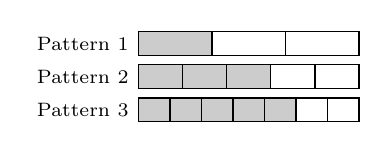
\begin{tikzpicture}[baseline=(current bounding box.north)]
  \foreach \p/\y in {1/0,2/-0.42,3/-0.84} {
    \node[font=\scriptsize,left] at (0,\y+0.15) {Pattern \p};
    \begin{scope}[shift={(0,\y)}]\fracbar{\p}\end{scope}}
  \end{tikzpicture}\end{minipage}
  \begin{enumerate}[start=2]
  \item \ealpara{Który \ealkeytr{wzór} ma $0.92$ swojego paska \ealkeytr{zacieniowanego}?}{Which \ealkey{pattern} has $0.92$ of its bar \ealkey{shaded}?}
    \workspace{1.0cm}
  \item \ealpara{Czy istnieje \ealkeytr{wzór} z $0.95$ swojego paska \ealkeytr{zacieniowanego}?}{Is there a \ealkey{pattern} with $0.95$ of its bar \ealkey{shaded}?}
    \ealpara{Wyjaśnij.}{Explain.}
    \vspace{0.8cm}\par\hrulefill
  \item \ealpara{Co dzieje się z \ealkeytr{ułamkiem} \ealkeytr{zacieniowanym}, gdy $n$ się zwiększa?}{What happens to the \ealkey{fraction} \ealkey{shaded} as $n$ gets larger?}
    \ealpara{Użyj rysunku, aby wyjaśnić, dlaczego nigdy nie osiąga 1.}{Use the picture to explain why it never reaches 1.} \hrulefill
  \end{enumerate}

% 360/n = 600/(n+20), 360(n+20) = 600n, 360n+7200 = 600n, 7200 = 240n,
% n = 30. Each person pays 12 pounds on both.
\item \ealpara{Wynajem minibusa kosztuje \pounds360, a autokaru \pounds600.}{A minibus costs \pounds360 to hire and a coach costs \pounds600.}
\ealpara{Na wycieczce autokar wiezie o 20 więcej osób niż minibus, a każda osoba płaci tę samą kwotę.}{On a trip, the coach carries 20 more people than the minibus, and each person pays the same amount.}
\ealpara{Ile osób jedzie minibusem i ile płaci każda osoba?}{How many people go on the minibus, and how much does each person pay?}
\workspace{1.3cm}
\end{enumerate}

% ================================================================
\ealpara{Znajdowanie \ealkeytr{niewiadomego} \ealkeytr{wzoru na $n$-ty wyraz}}{Finding an \ealkey{unknown} \ealkey{$n$th term}}
\parttitle{4}{Finding an unknown \boldmath$n$th term}

\begin{keyidea}
\ealpara{\ealkeytr{Wzór na $n$-ty wyraz} \ealkeytr{ciągu liniowego} można zapisać jako $an+b$, gdzie $a$ i $b$ są liczbami.}{\ealkey{The $n$th term} of a \ealkey{linear} \ealkey{sequence} can be written as $an+b$, where $a$ and $b$ are numbers.}

\ealpara{Dwa znane \ealkeytr{wyrazy} dają dwa \ealkeytr{równania} z $a$ i $b$, nazywane \textbf{\ealkeytr{układem równań}}, ponieważ te same $a$ i $b$ spełniają oba \ealkeytr{równania}.}{Two known \ealkey{terms} give two \ealkey{equations} in $a$ and $b$, called \textbf{\ealkey{simultaneous equations}} because the same $a$ and $b$ make both \ealkey{equations} true.}

\ealpara{Gdy odejmujemy jedno \ealkeytr{równanie} od drugiego, $b$ się \ealkeytr{skracają}.}{When we subtract one \ealkey{equation} from the other, the $b$s \ealkey{cancel out}.}
\end{keyidea}

\begin{wex}{a stack of cups}
\ealpara{Stos 3 kubków ma 15\,cm wysokości, a stos 8 kubków ma 25\,cm wysokości.}{A stack of 3 cups is 15\,cm tall, and a stack of 8 cups is 25\,cm tall.}
\ealpara{Wysokość stosu $n$ kubków wynosi $an+b$ centymetrów.}{The height of a stack of $n$ cups is $an+b$ centimetres.}
\ealpara{Znajdź \ealkeytr{wzór na $n$-ty wyraz}.}{Find the \ealkey{$n$th term}.}\par\smallskip
\eqlayout{0.3}
  {\centering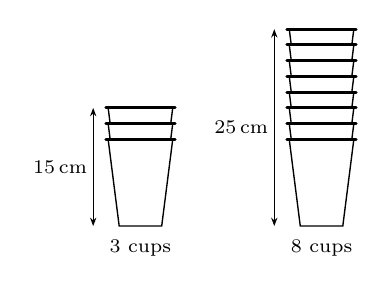
\begin{tikzpicture}[baseline=(current bounding box.center)]
    \cupstack{3}\stackheight{-0.6}{1.5}{15\,cm}
    \begin{scope}[shift={(2.3,0)}]\cupstack{8}\stackheight{-0.6}{2.5}{25\,cm}\end{scope}
    \node[font=\scriptsize,below] at (0,-0.05) {3 cups};
    \node[font=\scriptsize,below] at (2.3,-0.05) {8 cups};
  \end{tikzpicture}}
  {\begin{minipage}{\linewidth}
   \begin{minipage}[t]{0.5\linewidth}
   $\begin{array}[t]{@{}l@{\quad}r@{\;}c@{\;}l@{\quad}l@{}}
     \text{3 cups:} & 3a+b & = & 15 & (1)\\
     \text{8 cups:} & 8a+b & = & 25 & (2)
   \end{array}$\par\smallskip
   \ealpara{Odejmij (1) od (2):}{Subtract (1) from (2):}\par\smallskip
   \hspace*{1.2cm}\begin{working}
     5a & = & 10\\ \bsop{\div 5}
     a & = & 2
   \end{working}
   \end{minipage}\hfill
   \begin{minipage}[t]{0.48\linewidth}
   \ealpara{\ealkeytr{Podstaw} $a=2$ do (1):}{\ealkey{Substitute} $a=2$ into (1):}\par\smallskip
   \hspace*{0.6cm}\begin{working}
     3\times2+b & = & 15\\
     6+b & = & 15\\ \bsop{-6}
     b & = & 9
   \end{working}
   \end{minipage}
   \end{minipage}}
  {\ealpara{\ealkeytr{Wzór na $n$-ty wyraz} to \textbf{\boldmath$2n+9$}.}{The \ealkey{$n$th term} is \textbf{\boldmath$2n+9$}.}
   \ealpara{Każdy kubek dodaje 2\,cm do wysokości.}{Each cup adds 2\,cm to the height.}
   \ealpara{Sprawdź za pomocą (2): $8\times2+9=25$.}{Check with (2): $8\times2+9=25$.}}
\end{wex}

\begin{enumerate}[resume]
% 4a+b = 115, 10a+b = 175, 6a = 60, a = 10, 40+b = 115, b = 75. The nth
% term is 10n+75. (b) 10n+75 = 205, n = 13.
\item \ealpara{Stos 4 krzeseł ma 115\,cm wysokości, a stos 10 krzeseł ma 175\,cm wysokości.}{A stack of 4 chairs is 115\,cm tall, and a stack of 10 chairs is 175\,cm tall.}
\ealpara{Znajdź \ealkeytr{wzór na $n$-ty wyraz} na wysokość stosu $n$ krzeseł.}{Find the \ealkey{$n$th term} for the height of a stack of $n$ chairs.}\par\smallskip
\eqlayout{0.3}
  {\centering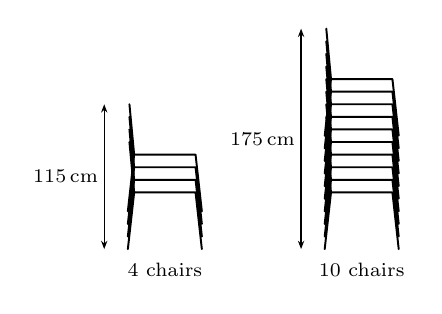
\begin{tikzpicture}[baseline=(current bounding box.center)]
    \chairstack{4}\stackheight{-0.3}{1.84}{115\,cm}
    \begin{scope}[shift={(2.5,0)}]\chairstack{10}\stackheight{-0.3}{2.80}{175\,cm}\end{scope}
    \node[font=\scriptsize,below] at (0.47,-0.05) {4 chairs};
    \node[font=\scriptsize,below] at (2.97,-0.05) {10 chairs};
  \end{tikzpicture}}
  {\begin{minipage}{\linewidth}
   \begin{minipage}[t]{0.5\linewidth}
   $\begin{array}[t]{@{}l@{\quad}r@{\;}c@{\;}l@{\quad}l@{}}
     \text{4 chairs:} & \sidegap[1.4cm] & = & \sidegap[1cm] & (1)\\
     \text{10 chairs:} & \sidegap[1.4cm] & = & \sidegap[1cm] & (2)
   \end{array}$\par\smallskip
   \ealpara{Odejmij (1) od (2):}{Subtract (1) from (2):}\par\smallskip
   \hspace*{1.2cm}\begin{working}
     \sidegap[1.2cm] & = & \sidegap[1cm]\\ \bsop{\div 6}
     a & = & \sidegap[1cm]
   \end{working}
   \end{minipage}\hfill
   \begin{minipage}[t]{0.48\linewidth}
   \ealpara{\ealkeytr{Podstaw} $a=$ \gap\ do (1):}{\ealkey{Substitute} $a=$ \gap\ into (1):}\par\smallskip
   \hspace*{0.6cm}\begin{working}
     \sidegap[1.4cm] & = & \sidegap[1cm]\\
     \sidegap[1.4cm] & = & \sidegap[1cm]\\ \bsop{-40}
     b & = & \sidegap[1cm]
   \end{working}
   \end{minipage}
   \end{minipage}}
  {\ealpara{\ealkeytr{Wzór na $n$-ty wyraz} to \ansline[2cm].}{The \ealkey{$n$th term} is \ansline[2cm].}
   \ealpara{Każde krzesło dodaje \gap\,cm do wysokości.}{Each chair adds \gap\,cm to the height.}
   \ealpara{Sprawdź za pomocą (2): \ansline[3cm].}{Check with (2): \ansline[3cm].}}\par\medskip
\ealpara{Ile krzeseł jest w stosie o wysokości 2.05\,m?}{How many chairs are in a stack that is 2.05\,m tall?}
\workspace{0.6cm}

% (a) 3a+5 = 2b+6 gives 3a-2b = 1, and (a+5)+(b+6) = 18 gives a+b = 7.
% (b) 2a+2b = 14, add: 5a = 15, a = 3, b = 4. (c) 8, 11, 14, 17, 20
% and 10, 14, 18, 22, 26. (d) 4a+5 = 4b+6 gives 4(a-b) = 1, but
% 4(a-b) is a multiple of 4 when a and b are whole numbers.
\newpage
\item \ealpara{Dwa \ealkeytr{ciągi liniowe} mają \ealkeytr{wzory na $n$-ty wyraz} $an+5$ i $bn+6$.}{Two \ealkey{linear} \ealkey{sequences} have \ealkey{$n$th terms} $an+5$ and $bn+6$.}
\ealpara{3. \ealkeytr{wyraz} $an+5$ jest równy 2. \ealkeytr{wyrazowi} $bn+6$, a 1. \ealkeytr{wyrazy} obu \ealkeytr{ciągów} sumują się do 18.}{The 3rd \ealkey{term} of $an+5$ is equal to the 2nd \ealkey{term} of $bn+6$, and the 1st \ealkey{terms} of the two \ealkey{sequences} add up to 18.}
\begin{enumerate}
\item \ealpara{Pokaż, że $3a-2b=1$ i $a+b=7$.}{Show that $3a-2b=1$ and $a+b=7$.} \hrulefill
\item \ealpara{\ealkeytr{Rozwiąż} \ealkeytr{układ równań}, aby znaleźć $a$ i $b$.}{\ealkey{Solve} the \ealkey{simultaneous equations} to find $a$ and $b$.}
  \ealpara{Najpierw pomnóż $a+b=7$ przez 2, aby $b$ się \ealkeytr{skróciły}, gdy dodamy \ealkeytr{równania}.}{Multiply $a+b=7$ by 2 first, so that the $b$s \ealkey{cancel out} when we add the \ealkey{equations}.}
  \workspace{2.8cm}
\item \ealpara{Zapisz pierwsze pięć \ealkeytr{wyrazów} każdego \ealkeytr{ciągu}.}{Write the first five \ealkey{terms} of each \ealkey{sequence}.} \hfill \ansline[4cm] \quad \ansline[4cm]
\item \ealpara{Wyjaśnij, dlaczego gdy $a$ i $b$ są \ealkeytr{liczbami całkowitymi nieujemnymi}, 4. \ealkeytr{wyrazy} $an+5$ i $bn+6$ nigdy nie mogą być równe.}{Explain why, when $a$ and $b$ are \ealkey{whole numbers}, the 4th \ealkey{terms} of $an+5$ and $bn+6$ can never be equal.} \hrulefill
\end{enumerate}

% 3p+4q = 138, 5p+6q = 222. 9p+12q = 414 and 10p+12q = 444, so p = 30
% and q = 12.
\item \ealpara{W centrum ogrodniczym C płot z 3 paneli kosztuje \pounds138, a płot z 5 paneli kosztuje \pounds222.}{At garden centre C, a fence of 3 panels costs \pounds138 and a fence of 5 panels costs \pounds222.}
\ealpara{Każdy płot ma o jeden słupek więcej niż paneli, jak w Q8.}{Each fence has one more post than panels, as in Q8.}
\ealpara{Znajdź koszt jednego panelu i koszt jednego słupka.}{Find the cost of one panel and the cost of one post.}
\workspace{3.0cm}

% x+y, x+2y, 2x+3y, 3x+5y. 2x+3y = 31 and 3x+5y = 50 give x = 5 and
% y = 7: 5, 7, 12, 19, 31, 50.
\item \ealpara{W \ealkeytr{ciągu typu Fibonacciego} każdy \ealkeytr{wyraz} jest \ealkeytr{sumą} dwóch poprzednich \ealkeytr{wyrazów}.}{In a \ealkey{Fibonacci-type sequence}, each \ealkey{term} is the \ealkey{sum} of the two \ealkey{terms} before it.}
\ealpara{Uzupełnij tabelę, a następnie znajdź $x$ i $y$, gdy 5. \ealkeytr{wyraz} wynosi 31, a 6. \ealkeytr{wyraz} wynosi 50.}{Complete the table, then find $x$ and $y$ when the 5th \ealkey{term} is 31 and the 6th \ealkey{term} is 50.}\par\smallskip
{\setlength{\tabcolsep}{3pt}\renewcommand{\arraystretch}{1.3}%
\begin{tabular}{|l|*{6}{C{1.5cm}|}}\hline
{\small \ealkey{Term}} & 1st & 2nd & 3rd & 4th & 5th & 6th\\\hline
{\small Value}\rowstrut & $x$ & $y$ & $x+y$ & & & \\\hline
\end{tabular}}
\workspace{2.6cm}

% Open. 3n+12 = 5n-2 gives n = 7. For example, Kai has 4 more boxes
% than Lily, with 3 pens in each, and Lily has n boxes of 5 pens but
% has given away 2 pens.
\item \ealpara{Zapisz zadanie z życia codziennego o dwóch \ealkeytr{ciągach}, które prowadzi do \ealkeytr{równania} $3(n+4)=5n-2$.}{Write a real-life problem about two \ealkey{sequences} that leads to the \ealkey{equation} $3(n+4)=5n-2$.}
\ealpara{Następnie \ealkeytr{rozwiąż} swoje zadanie.}{Then \ealkey{solve} your problem.}
\par\vspace{2.2cm}\hrulefill\par\vspace{9pt}\hrulefill

% (a) Open. For example 4n+7 and 97-5n. (b) No. If an+b = cn+d when
% n = 10 and when n = 20, subtracting gives 10a = 10c, so a = c and
% then b = d, and the two sequences are the same.
\item
\begin{enumerate}
\item \ealpara{Zaprojektuj dwa \ealkeytr{ciągi}, jeden rosnący i jeden malejący, które są równe na 10. \ealkeytr{wyrazie} o wartości 47.}{Design two \ealkey{sequences}, one that goes up and one that goes down, that are equal at the 10th \ealkey{term} with the value 47.}
  \ealpara{Zapisz ich \ealkeytr{wzory na $n$-ty wyraz}.}{Write their \ealkey{$n$th terms}.} \hfill
  \ansline[2.6cm] \quad \ansline[2.6cm]
\item \ealpara{Dwa różne \ealkeytr{ciągi liniowe} mają równe 10. \ealkeytr{wyrazy}.}{Two different \ealkey{linear} \ealkey{sequences} have equal 10th \ealkey{terms}.}
  \ealpara{Czy mogą mieć także równe 20. \ealkeytr{wyrazy}?}{Can they also have equal 20th \ealkey{terms}?}
  \ealpara{Wyjaśnij.}{Explain.}\par\vspace{1.9cm}\hrulefill
\end{enumerate}
\end{enumerate}

\end{document}